\section{植物与水分}

\subsection{概述}

\subsubsection{水在植物体内的存在形式}

组织含水量的变化受植物种类、器官类型、不同生境的影响。通常生命活动较旺盛的组织含水量较高。

植物体内的水分为束缚水(结合水)和自由水两类:

\begin{description}
	\item[束缚水] 靠近蛋白质胶粒而被吸附的水分,不起溶剂作用,与抗逆性相关。
	\item[结合水] 可自由流动,起溶剂作用,与代谢强度有关。
\end{description}

\subsubsection{细胞间的水分交换}

细胞间存在两侧水势差时,水分子的运动包括:
\begin{description}
	\item[水分子的跨膜扩散] 由浓度梯度推动的,水分子直接跨过细胞膜的过程。
	\item[通过水孔蛋白的集流] 由水势差推动的,通过水孔蛋白介导的跨膜过程。
\end{description}

\paragraph{水孔蛋白}

水孔蛋白的单体由6次跨膜的$\upalpha$螺旋围成一个通道,4个单体组成一个水孔蛋白。水孔蛋白中研究最多的两类是质膜内在蛋白(PIP)和液泡膜内在蛋白(TIP)。

水孔蛋白的表达有以下特点:
\begin{description}
	\item[时空性] 发育中的组织表达量高;根尖表达量比成熟区高;TIP和PIP在根中比叶片中表达量高。
	\item[日夜节律性] 白天蒸腾强烈时表达量更高。
\end{description}

\subsection{水势}

\subsubsection{水势的计算}

水势由压力势($\psi_{\text{p}}$)、渗透势($\psi_{\uppi}$)、衬质势($\psi_{\text{m}}$)三部分组成。即\[\psi_{\text{w}}=\psi_{\text{p}}+\psi_{\uppi}+\psi_{\text{m}}\]

\begin{description}
	\item[压力势] 植物细胞吸水产生膨压,细胞壁因此产生的反作用力可阻碍吸水,这就是压力势。正常植物细胞内$\psi_{\text{p}}<0$,因为细胞壁挤压原生质体阻碍吸水;蒸腾作用下可出现$\psi_{\text{p}}>0$
	\item[渗透势] 体系内水溶质颗粒的存在导致的水势改变量,又称溶质势。$\psi_{\uppi}\approx-i\alpha CRT$,其中:
	\begin{description}
		\item[i] 溶质的范特霍夫系数,即溶质解离成几个部分,非电解质$i=1$;
		\item[$\alpha$] 溶质颗粒的活度系数,根据实验测得;
		\item[$C$] 溶质颗粒的摩尔浓度;
		\item[$R$] 理想气体常数;
		\item[$T$] 绝对温度,单位是开;
	\end{description}
	\item[衬质势] 亲水物质表面对水的吸附作用,在有大液泡的细胞内,衬质势常可忽略。
\end{description}

\begin{qj}[:植物细胞水势变化]
	常有题目考察: 把细胞放进某溶液中,问细胞内水势如何变化。答案是:若该溶液比细胞内水势高,则细胞内水势、渗透势、压力势都变高;反之则变低。概括为:“\textbf{高就高,低就低}”。
\end{qj}

\subsubsection{小液流法测定水势}

把植物组织(如叶)浸泡在不同浓度的蔗糖溶液当中,会出现以下情况:
\begin{itemize}
	\item 植物水势较高,则植物失水、溶液得水,溶液密度下降,植物下沉;
	\item 植物水势较低,则植物得水、溶液失水,溶液密度上升,植物上升;
	\item 植物水势等于溶液水势,则植物不动。
\end{itemize}

\section{植物的矿质营养}

\subsection{植物必需的矿质元素}

将植物体彻底燃烧后的灰烬中存在的元素,称为\sy{灰分元素}。氮并不在其中,但是\zhongdian{氮在土壤中是以盐离子的形式被吸收},故把氮加入到\sy{矿质元素}之列。

植物常见矿质元素缺乏症列于\autoref{tab:植物矿质营养缺乏症}中。

\begin{table}[htbp]
	\centering
	\begin{tabularx}{\textwidth}{|C|c|c|c|c|c|}
		\hline
		\textbf{元素} & 根 & 茎 & 叶 & 生殖 & 参与过程 \\ \hline
		\textbf{氮} &  & 矮小分枝少 & 小、色淡或红 & 花小 & “生命元素” \\ \hline
		\textbf{磷} & 横向生长\footnotemark & 矮小分枝少 & 小、暗绿或红 & 迟熟 & 蛋白质合成 \\ \hline
		\textbf{钾} &  & 柔弱易倒伏 & 边缘焦枯 &  & “品质元素” \\ \hline
		\textbf{硫} &  & 同氮 &  &  & 酶的合成 \\ \hline
		\textbf{钙} & 停止伸长 & 幼嫩器官死 &  &  & 第二信使、壁 \\ \hline
		\textbf{镁} &  &  & 脉间失绿 &  & 酶、叶绿素 \\ \hline
		\textbf{铁} &  &  & 脉间失绿 &  & 电子传递 \\ \hline
		\textbf{锰} &  &  & 脉间失绿 &  & 活化酶 \\ \hline
		\textbf{硼} &  &  &  & 花而不实 & 壁、生殖 \\ \hline
		\textbf{锌} &  & 节间短 & 小、缺绿 &  & Trp合成 \\ \hline
		\textbf{铜} &  &  & 嫩叶尖始黑绿 &  & 酶、电子传递 \\ \hline
		\textbf{钼} &  &  & 脉间失绿 &  & 氮代谢 \\ \hline
		\textbf{氯} & 生长慢 &  & 小、枯、黄 &  & 光解水 \\ \hline
		\textbf{镍} &  &  & 尖部脲积累 &  & 脲酶、氢化酶 \\ \hline
	\end{tabularx}
	\caption{植物矿质营养缺乏症}
	\label{tab:植物矿质营养缺乏症}
\end{table}
\footnotetext{指的是侧根和根毛生长。}

在上述元素中,
\begin{itemize}
	\item 易移动的有:磷、氮、氯、钼、镁、锌、钾,缺素症先出现于老叶;
	\item 不易移动的有:钙、铁、硼、铜、锰\footnote{锰在不同植物中的移动性不同。}、硫、硅、镍、钠,缺素症先出现于新叶。
\end{itemize}

\begin{qj}[:易移动的元素记忆法]
	上述易移动的元素可按顺序,谐音为:林丹绿幕美新甲。意思是,林丹在绿幕前,做新的美甲。
\end{qj}

另外,把硅、钠、钴称为有益元素:

\begin{itemize}
	\item 硅以\ce{H3SiO4}吸收,有利于禾本科作物发育,\ce{SiO2}的水合物参与细胞壁的构成。缺乏会导致倒伏;
	\item \ce{Na+}在\ce{C4}和CAM植物中参与催化PEP再生,促进维管束鞘和叶肉细胞之间的丙酮酸运输。缺乏导致黄化、坏死、不开花;
	\item \ce{Co+}是维生素B$_{12}$的成分,参与催化豆血红蛋白的合成,与固氮相关。
\end{itemize}

植物的必需矿质元素见表\autoref{tab:植物利用的元素及其形式},其中右侧的元素为微量元素。

\begin{table}[htbp]
	\centering
	\begin{tabularx}{\textwidth}{|>{\centering\arraybackslash}m{3em}|C||>{\centering\arraybackslash}m{3em}|C|}
		\hline
		\textbf{元素} & \textbf{植物的利用形式} & \textbf{元素} & \textbf{植物的利用形式} \\ \hline
		碳  & $ \mathrm{CO_2} $                & 氯  & $ \mathrm{Cl^-} $                \\ \hline
		氧  & $ \mathrm{O_2}, \mathrm{H_2O}, \mathrm{CO_2} $       & 铁  & $ \mathrm{Fe^{3+}}, \mathrm{Fe^{2+}} $        \\ \hline
		氢  & $ \mathrm{H_2O} $                & 锰  & $ \mathrm{Mn^{2+}} $               \\ \hline
		氮  & $ \mathrm{NO_3^-}, \mathrm{NH_4^+} $        & 硼  & $ \mathrm{BO_3^{3-}} $              \\ \hline
		钾  & $ \mathrm{K^+} $                 & 锌  & $ \mathrm{Zn^{2+}} $               \\ \hline
		钙  & $ \mathrm{Ca^{2+}} $               & 铜  & $ \mathrm{Cu^{2+}} $               \\ \hline
		镁  & $ \mathrm{Mg^{2+}} $               & 镍  & $ \mathrm{Ni^{2+}} $               \\ \hline
		磷  & $ \mathrm{H_2PO_4^-}, \mathrm{HPO_4^{2-}} $    & 钼  & $ \mathrm{MoO_4^{2-}} $             \\ \hline
		硫  & $ \mathrm{SO_4^{2-}} $              &  &  \\ \hline
	\end{tabularx}
	\caption{植物利用的元素及其形式}
	\label{tab:植物利用的元素及其形式}
\end{table}

\subsection{氮、硫、磷的同化}

\subsubsection{氮同化}

氮同化有两个路径,
\begin{enumerate}
	\item 植物自己吸收$\mathrm{NO_{3}^{-}}\xrightarrow{\text{硝酸还原酶、亚硝酸还原酶}}\mathrm{NH_{4}^{+}}$,或直接吸收$\mathrm{NH_{4}^{+}}$;
	\item 依靠共生固氮菌产生的$\mathrm{NO_{3}^{-}}$。
\end{enumerate}

\paragraph{硝酸盐的还原}

植物通过质膜上的硝酸盐-质子同向转运体(NRT)转运$\mathrm{NO_{3}^{-}}$,该转运体受$\mathrm{NO_{3}^{-}}$诱导表达。

\subparagraph{第一步:硝酸盐$\longrightarrow$亚硝酸盐}

该反应受硝酸还原酶的催化,主要存在于高等植物的根和叶中。硝酸还原酶是诱导酶。

整个反应过程从NAD(P)H开始,经过FAD、细胞色素$_{557}$、Mo辅因子,最后把电子交给$\mathrm{NO_{3}^{-}}$,同时生成一分子水。

\subparagraph{第二步:亚硝酸盐$\longrightarrow$铵盐}

该反应由亚硝酸还原酶(NiR)催化,电子供体为铁氧还蛋白Fd$_{\text{red}}$。NiR的\zhongdian{辅基是铁硫簇(\ce{Fe4S4})和血红素}。(\autoref{fig:亚硝酸还原酶的机理},其中Heme代表血红素)

\begin{figure}[htbp]
	\centering
	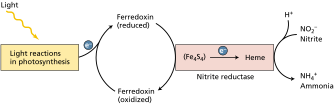
\includegraphics[width=\textwidth]{亚硝酸还原酶的机理.pdf}
	\caption{亚硝酸还原酶的机理}
	\label{fig:亚硝酸还原酶的机理}
\end{figure}

\paragraph{氨(铵)同化}

植物体内的氨将立刻被同化,因为氨会抑制呼吸链电子传递。

氨同化包括下面三个途径:

\begin{description}
	\item[谷氨酰胺合成酶途径] 铵+谷氨酸$\xrightarrow{\text{GS}}$谷氨酰胺,谷氨酰胺+$\alpha$-酮戊二酸$\xrightarrow{\text{GOGAT}}$谷氨酰胺;
	\item[谷氨酸脱氢酶途径] 铵+$\alpha$-酮戊二酸$\xrightarrow[\text{NA(D)PH}]{\text{GDH}}$谷氨酸;
	\item[氨基交换作用] 谷氨酸和谷氨酰胺把氨基转移给别的酮酸,生成新的氨基酸的过程。
\end{description}

\paragraph{生物固氮}

生物固氮主要通过两类微生物实现,独立生存的和共生的。

独立生存的包括下面三类:

\begin{itemize}
	\item 好气性细菌,如固氮菌属;
	\item 嫌气性细菌,如梭菌属;
	\item 蓝藻。
\end{itemize}

共生的例如下面三类:

\begin{itemize}
	\item 根瘤菌——与豆科共生;
	\item 放线菌——与非豆科植物共生;
	\item 鱼腥藻(属于蓝藻)——与满江红(红萍)共生。
\end{itemize}

固氮微生物体内都有\sy{固氮酶}(\autoref{fig:固氮酶的机理})。固氮酶催化氮气变为氨,\zhongdian{每转换一分子\ce{N2}消耗16分子ATP}。

\begin{figure}[htbp]
	\centering
	\includegraphics[width=0.8\linewidth]{固氮酶}
	\caption{固氮酶的机理}
	\label{fig:固氮酶的机理}
\end{figure}


固氮酶有两个组分:铁蛋白和钼铁蛋白。

\begin{description}
	\item[铁蛋白] 较小,两个亚基。每个亚基含有一个\ce{Fe4S4}簇,用于水解ATP、还原钼铁蛋白。
	\item[钼铁蛋白] 较大,四个亚基,每个亚基含有两个Mo-Fe-S簇,用于还原\ce{N2}。
\end{description}

固氮酶怕\ce{O2},但ATP需要呼吸作用提供。解决这一矛盾的方式有:

\begin{itemize}
	\item 独立生活的固氮细菌保留无氧生活周期;
	\item 蓝细菌形成异形胞;
	\item 豆科植物合成豆血红蛋白。
\end{itemize}


\subsubsection{硫同化}



\section{光合作用}

\subsection{光合色素}

\subsubsection{光合色素的化学特性}

高等植物的光合色素有两类:类胡萝卜素和叶绿素,排列在类囊体膜上。

\paragraph{叶绿素}

叶绿素主要分为叶绿素a和叶绿素b两类。叶绿素a呈蓝绿色,叶绿素b呈黄绿色。它们能溶于有机溶剂。



叶绿素是叶绿酸和甲醇、叶绿醇发生酯化反应形成的。(\autoref{fig:cholorophyll})

\begin{figure}[htbp]
	\centering
	\includegraphics[width=0.9\linewidth]{Pics/叶绿素a和叶绿素b}
	\caption{叶绿素a和叶绿素b的结构}
	\label{fig:cholorophyll}
\end{figure}

叶绿素拥有亲水的金属卟啉环“头部”和疏水的叶绿醇“尾巴”。疏水的尾巴可以把叶绿素固定在类囊体膜上,亲水的头部有利于和蛋白质结合。

绝大部分叶绿素a分子和全部叶绿素b分子承担收集和传递光能的功能。少数特殊叶绿素a对承担把光能转换为化学能的功能。

\paragraph{类胡萝卜素}

叶绿体中的类胡萝卜素主要有叶黄素和$\beta$-胡萝卜素两种。叶黄素是胡萝卜素衍生的醇类。它们是重要的抗氧化剂。叶黄素呈黄色,类胡萝卜素呈橙黄色。

类胡萝卜素也有传递光能的作用,还可保护光合机构免受过剩光能伤害,如叶黄素循环。

\subsubsection{光合色素的光学特性}

\paragraph{两个吸光强区}

叶绿素主要吸收红光和蓝紫光。叶片的反射光和透射光都是绿色,叶绿素溶液也呈绿色。叶绿素溶液的荧光是红色的。(\autoref{fig:yelvsurongye})

\begin{figure}[htbp]
	\centering
	\begin{subfigure}{0.45\textwidth}
		\includegraphics[width=\linewidth]{叶绿素溶液2}
	\end{subfigure}
	\hfill
	\begin{subfigure}{0.45\textwidth}
		\includegraphics[width=\linewidth]{叶绿素溶液3}
	\end{subfigure}
	\caption{叶绿素溶液的透射光和反射光}
	\label{fig:yelvsurongye}
\end{figure}


类胡萝卜素主要吸收蓝紫光,不吸收红光。

\paragraph{激发态}

叶绿素分子吸收光能后,就由基态上升为激发态。激发态不稳定,停留时间非常短,以后就迅速向低能状态转变。转变的途径有:(\autoref{fig:yelvsu_light_absorb})
\begin{itemize}
	\item 以热的形式回到基态;
	\item 以荧光或磷光返回基态。荧光是从第一单线态返回时发出的光,磷光是由第一三线态返回时发出的光。磷光寿命更长。
	\item 激发态的叶绿素参与能量转移,迅速传递光能。
\end{itemize}

\begin{figure}[htbp]
	\centering
	\includegraphics{叶绿素吸收光之后的能量转变}
	\caption{叶绿素吸收光之后的能量转变}
	\label{fig:yelvsu_light_absorb}
\end{figure}


\subsubsection{叶绿素的合成和降解}

\paragraph{叶绿素的合成}

叶绿素的前体是谷氨酸。反应分为四个阶段:
\begin{enumerate}
	\item 谷氨酸$\longrightarrow$5-氨基酮戊酸$\longrightarrow$卟胆原;
	\item 4个卟胆原$\longrightarrow$原卟啉IX$\xrightarrow{\ce{Mg^{2+}}}$Mg原卟啉$\longrightarrow$单乙烯基原叶绿素酯a;
	\item 单乙烯基原叶绿素酯a$\xrightarrow{\text{NADPH、光}}$叶绿素酯a;
	\item 叶绿素酯a$\xrightarrow{植醇尾巴}$叶绿素a。
\end{enumerate}

叶绿素b是由叶绿素a演变来的。

\paragraph{叶绿素的降解}

叶绿素b$\longrightarrow$叶绿素a$\longrightarrow$脱植基叶绿素a$\longrightarrow$脱镁叶绿素a$\longrightarrow$水溶性无色产物,进入液泡。

\paragraph{植物的叶色}

植物的叶色是各种色素的综合表现。

\begin{itemize}
	\item 正常植物呈绿色:叶绿素比类胡萝卜素多;
	\item 秋天呈红色:气温降低,叶绿素分解,显示出类胡萝卜素的颜色。
	\item 枫树变红:积累糖分御寒,利用糖分合成红色的花色素苷。
\end{itemize}

因此,影响光合色素合成的因素可以影响植物的叶色:

\begin{description}
	\item[光] 叶绿素合成需要光。一般植物在黑暗中无法合成叶绿素,导致黄化。
	\item[温度] 温度影响酶的活性。
	\item[矿质元素] 氮和镁是组成叶绿素的元素。一些金属离子是叶绿素合成有关酶的活化剂。
\end{description}

\subsection{光合作用过程}

\subsubsection{原初反应}

\subsubsection{电子传递}

S态转换机制

\autoref{fig:S态转换机制}
\begin{figure}[htbp]
	\centering
	\includegraphics[width=\linewidth]{S态转换机制.png}
	\caption{S态转换机制}
	\label{fig:S态转换机制}
\end{figure}

\subsubsection{碳同化}

\paragraph{C$_{3}$途径}

\paragraph{C$_{4}$途径}

\paragraph{CAM途径}


\begin{table}[htbp]
	\centering
	\begin{tabularx}{\textwidth}{|c|C|C|C|}
		\hline
		特征 & C$_3$ 植物 & C$_4$ 植物 & CAM 植物 \\ 
		\hline
		分布 
		& 温带 
		& 热带、亚热带 
		& 干旱地区 \\ 
		\hline
		生物产量
		& 中 
		& 高 
		& 低 \\ 
		\hline
		叶结构 
		& \begin{tabular}[c]{@{}c@{}}无花环,\\一种叶绿体\end{tabular}
		& \begin{tabular}[c]{@{}c@{}}有花环,\\两种叶绿体\end{tabular} 
		& \begin{tabular}[c]{@{}c@{}}无花环,\\一种叶绿体\end{tabular} \\ 
		\hline
		叶绿素 a/b 
		& 中 
		& 高
		& 低\\ 
		\hline
		CO$_2$ 固定酶 
		& Rubisco 
		& PEPC、Rubisco 
		& PEPC、Rubisco \\ 
		\hline
		CO$_2$ 固定途径 
		& C$_{3}$ 
		& C$_4$和C$_{3}$分空间 
		& CAM和C$_{3}$分时段 \\ 
		\hline
		CO$_2$受体 
		& RuBP 
		& PEP 
		& \begin{tabular}[c]{@{}c@{}}光下RuBP\\暗中PEP\end{tabular} \\ 
		\hline
		固碳初产物 
		& PGA 
		& OAA 
		& \begin{tabular}[c]{@{}c@{}}光下PGA\\暗中OAA\end{tabular} \\ 
		\hline
		PEP 羧化酶活性
		& 低 
		& 高 
		& 中 \\ 
		\hline
		光合速率
		& 中 
		& 高 
		& 低 \\ 
		\hline
		CO$_2$补偿点 
		& 高
		& 中 
		& 低 \\ 
		\hline
		光饱和点 
		& 全日照的一半 
		& 无 
		& 无 \\ 
		\hline
		光合最适温度
		& 低 
		& 高 
		& 高 \\ 
		\hline
		蒸腾比率
		& 高
		& 中 
		& 低 \\ 
		\hline
		气孔张开 
		& 白天 
		& 白天 
		& 晚上 \\ 
		\hline
		光呼吸 
		& 高 
		& 低 
		& 低 \\ 
		\hline
		耐旱性 
		& 弱 
		& 强 
		& 极强 \\ 
		\hline
	\end{tabularx}
	\caption{C$_3$/C$_4$/CAM 植物主要光合与生理特征比较}
	\label{tab:photosynthesis_comparison}
\end{table}

\subsection{光呼吸}

\begin{figure}[htbp]
	\centering
	\includegraphics[width=0.5\textwidth]{光呼吸}
	\caption{光呼吸}
	\label{fig:光呼吸}
\end{figure}



\section{植物同化物的运输}

\subsection{概述:运输的途径和方向}

\subsubsection{运输途径}

\begin{description}
	\item[短距离运输] 同化物在细胞内或细胞之间的运输;
	\item[长距离运输] 同化物经维管系统,从源到库的运输。
\end{description}

\paragraph{短距离运输}

胞间连丝\autoref{fig:胞间连丝的结构}

\begin{figure}[htbp]
	\centering
	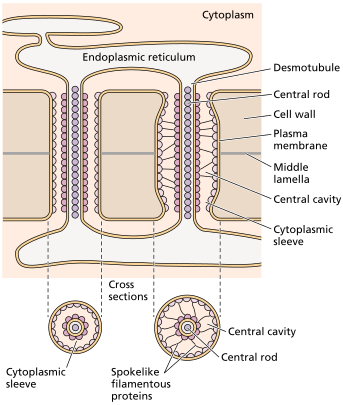
\includegraphics[width=0.7\linewidth]{胞间连丝的结构}
	\caption{胞间连丝的结构}
	\label{fig:胞间连丝的结构}
\end{figure}

\paragraph{长距离运输}

\subsection{韧皮部装载}

韧皮部运输的关键有二:
\begin{enumerate}
	\item 同化产物从“源”装入筛管,即韧皮部装载;
	\item 同化产物从筛管卸出到“库”,即韧皮部卸出。
\end{enumerate}

韧皮部装载的途径有三:
\begin{description}
	\item[质外体途径] 蔗糖从细胞壁穿过,进入筛管;
	\item[共质体途径] 蔗糖经胞间连丝进入筛管;
	\item[扩散] 依靠叶肉细胞和筛管之间的蔗糖浓度差,从胞间连丝扩散进入筛管。
\end{description}

\subsection{韧皮部卸出}

\subsection{韧皮部运输的机理}

\autoref{fig:压力流动学说}
\begin{figure}[htbp]
	\centering
	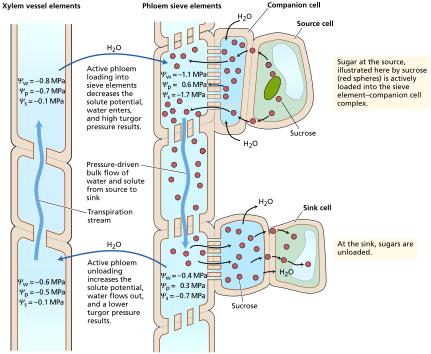
\includegraphics[width=1\linewidth]{压力流动学说}
	\caption{压力流动学说}
	\label{fig:压力流动学说}
\end{figure}

\section{植物次生代谢物}

\subsection{概述:初生代谢物和次生代谢物的区别}

\subsection{萜类}

\subsubsection{萜类的种类}

\sy{萜类}化合物的基本单位是异戊二烯,可以是链状或环状。单萜为两个异戊二烯单位合成,10个C原子。(\autoref{tab:萜类化合物的种类})

\begin{table}[htbp]
	\centering
	\begin{tabularx}{\textwidth}{|c|c|X|}
		\hline
		\textbf{类型} & \textbf{C} & \multicolumn{1}{c|}{\textbf{例子}} \\ \hline
		单萜 & 10 & 香叶醇、香叶醛、薄荷醇、薄荷酮、龙脑、樟脑、柠檬醛 \\ \hline
		倍半萜 & 15 & 法尼醇、\zhongdian{青蒿素}、\zhongdian{脱落酸}、姜烯、$\beta$-丁香烯、桉叶醇、$\alpha$-檀香烯 \\ \hline
		二萜 & 20 & \ \hspace{-0.25em}\zhongdian{植醇}、\zhongdian{维生素A}、银杏内酯、\zhongdian{紫杉醇}、甜菊苷、\zhongdian{赤霉素} \\ \hline
		三萜 & 30 & 甘草次酸、人参皂苷、熊果酸、\zhongdian{角鲨烯}、齐墩果酸、三萜醇/酸 \\ \hline
		四萜 & 40 & \ \hspace{-0.25em}{\color{blue}胡萝卜素}、\zhongdian{叶黄素} \\ \hline
		多萜 & $>$40 & 橡胶、杜仲胶 \\ \hline
	\end{tabularx}
	\caption{植物萜类化合物的种类}
	\label{tab:萜类化合物的种类}
\end{table}

\subsubsection{萜类的生物合成}

植物体内萜类合成有两条途径:

\begin{description}
	\item[甲羟戊酸途径(MVA)] 位于细胞质基质中。原料是3分子乙酰CoA,反应关键酶是HMG-CoA还原酶(HMGR),催化生成MVA\footnote{甲羟戊酸也被称为甲瓦龙酸。}。
	\item[甲基赤藓糖醇磷酸途径(MEP)] 位于质体中。原料是丙酮酸和3-磷酸甘油醛,反应关键酶是DXP还原异构酶(DXR),催化生成MEP。
\end{description}
两种途径最后都生成异戊烯基焦磷酸(IPP)和二甲丙烯焦磷酸(DMAPP),之后进一步合成萜类。IPP和DMAPP被称为“活化的异戊二烯”。

DMAPP+IPP$\longrightarrow$牻牛儿基焦磷酸(GPP,单萜前体)$\xrightarrow{\text{+IPP}}$法尼基焦磷酸(FPP,倍半萜和三萜前体)$\xrightarrow{\text{+IPP}}$牻牛儿牻牛儿基焦磷酸(GGPP,二萜和四萜前体)。(\autoref{fig:萜类合成途径})

\begin{figure}[htbp]
	\centering
	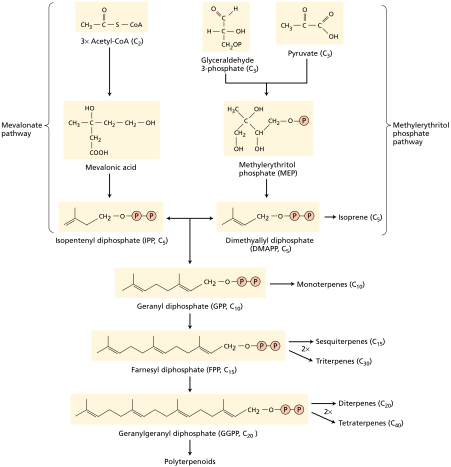
\includegraphics[width=\linewidth]{萜类合成途径}
	\caption{萜类合成途径}
	\label{fig:萜类合成途径}
\end{figure}

\subsection{酚类}

\subsubsection{酚类的种类}

酚类是芳香环上的氢原子被取代后的产物。\zhongdian{常见的酚类化合物有:水杨酸、香豆素、香豆酸、伞形酮、黄酮、花青素、木质素。}酚类的水溶性取决于其取代基。

\subsubsection{酚类的生物合成}

酚类化合物主要通过莽草酸途径合成其氨基酸前体。

\begin{itemize}
	\item 从4-磷酸赤藓糖(来自磷酸戊糖途径)和磷酸烯醇式丙酮酸(来自糖酵解)开始;
	\item 经过重要中间产物莽草酸$\xrightarrow{\text{多步反应}}$分支酸\footnote{这里的分支酸{\color{red}并非}分枝菌酸,二者有天壤之别}。
	\item 从分支酸可以合成Tyr、Phe、Trp三个具苯环的氨基酸。
\end{itemize}

苯丙素类和黄酮类的合成起始于Phe或Tyr。

木质醇在细胞质基质的合成起始于Phe,合成好之后在细胞壁中转化为木质素。

\subsection{次生含氮化合物}

次生含氮化合物种类很多,这里只介绍生物碱和含氰苷。

\subsubsection{生物碱}

除了蛋白质和核酸以及它们的前体,剩下的含氮化合物都可以称为生物碱。多数生物碱具有碱性,但是也有例外,如喜树碱、紫杉醇、秋水仙碱。

生物碱在较为进化的植物类群中存在较多,动物中也有但较少。生物碱含量一般很低,然而金鸡纳树皮中含12\%是个例外。

\subsubsection{含氰苷}

含氰苷本身无毒,存在于植物叶表皮细胞的液泡中。叶肉细胞中含有糖苷酶。一旦植物被啃食,这两种物质就会接触,生成糖和氰醇,氰醇再生成酮和氰化物。氰化物可抑制呼吸链复合体IV(细胞色素c氧化酶)。木薯中含有较多含氰苷。

\subsubsection{芥子油苷}

十字花科植物含有芥子油苷。芥子油苷被酶水解可生成有刺激性的物质,用以抵抗食草动物。

\section{植物细胞信号转导}

\subsection{跨膜信号转导}

在植物细胞中,\zhongdian{主要是双元系统(二元组分系统)和受体激酶介导的跨膜信号转导},小G蛋白在胞内信号转导发挥重要作用。三聚体G蛋白和GPCR则较少参与。

\subsubsection{双元系统}

细菌和植物都具有双元系统,其受体组成略有不同,详见\autoref{fig:细菌和植物的双元系统}。其中,HK段位于质膜,其余部分位于胞质。

\begin{figure}[htbp]
	\centering
	\includegraphics{细菌和植物的双元系统}
	\caption{细菌(A)和植物(B)的双元系统}
	\label{fig:细菌和植物的双元系统}
\end{figure}

目前已知,\zhongdian{细胞分裂素和乙烯的受体}采用双元系统来传递信号。

\subsubsection{受体激酶}

细胞表面的受体具有蛋白激酶的性质,称为受体激酶,或类受体蛋白激酶(RLK)。植物的RLK多属于丝氨酸/苏氨酸激酶。RLK由胞外结构区、跨膜螺旋区、胞内蛋白激酶催化区组成。

根据胞外结构域的结构,将RLK分为三类:

\begin{description}
	\item[含S结构域的RLK] 含有与调节油菜自交不亲和S糖蛋白同源的序列。
	\item[含富亮氨酸重复的RLK] 含有重复出现的亮氨酸。如\zhongdian{油菜素内酯的受体}。
	\item[类表皮生长因子的RLK] 含类似动物表皮生长因子的结构。
\end{description}

\subsection{细胞内信号转导网络}

\subsubsection{第二信使}

植物中发现的第二信使有\ce{Ca^{2+}}、脂质、pH变化、某些氧化还原剂如维生素C、谷胱甘肽、、过氧化氢等。

\paragraph{\ce{Ca^{2+}}/CaM}

静息时,细胞质基质的\ce{Ca^{2+}}很低,这有赖于钙泵和\ce{Ca^{2+}}-\ce{H+}反向转运体。在受到刺激后,胞质\ce{Ca^{2+}}会升高或区域分布变化。\ce{Ca^{2+}}与钙离子感应蛋白结合发挥作用。

植物细胞中发现的钙离子感应蛋白包括:钙调蛋白(CaM)、钙依赖型蛋白激酶(CDPK)、钙调磷酸酶B相似蛋白(CBL)。

钙调蛋白既可以直接与靶酶结合,调节酶的活性;也可以与\ce{Ca^{2+}}结合后再激活靶酶。细胞内外都存在CaM。

\paragraph{脂质信号分子}

已知的脂质信号分子包括磷脂酸(PA)、磷脂酰肌醇(PI)、鞘脂、溶血磷脂、N-酰基乙醇胺、脂肪酸等。

\sy{磷脂酶D}(PLD)可催化不同的磷脂水解产生PA、胆碱、乙醇胺等。

PI在PI激酶和PIP激酶的作用下形成PIP$_{2}$。PIP$_{2}$在磷脂酶C(PLC)催化下产生IP$_{3}$和DAG(二酰甘油)。IP$_{3}$可打开内质网和液泡膜上的配体门控\ce{Ca^{2+}}通道。但是,\zhongdian{植物基因组中尚未发现PKC基因},故DAG的第二信使作用存疑。\zhongdian{植物细胞的PLC通路与动物细胞相差很大}。

\subsubsection{蛋白质可逆磷酸化}

蛋白质可逆磷酸化依赖于各类蛋白激酶和蛋白磷酸酶。如MAPK级联反应。

\paragraph{蛋白激酶}

蛋白激酶可分为丝氨酸/苏氨酸激酶、酪氨酸激酶、组氨酸激酶三类,它们分别磷酸化底物对应的氨基酸残基。

钙依赖型蛋白激酶(CDPK)是植物特有的激酶,属于丝氨酸/苏氨酸激酶。CDPK的N端有激酶催化结构域,C端有\ce{Ca^{2+}}结合结构域,可同时起到钙离子感应蛋白和激酶的作用。

\paragraph{蛋白磷酸酶}

植物中丝氨酸/苏氨酸蛋白酶PP1和PP2在抗逆过程中发挥作用。植物中还发现了天冬氨酸特异性的半胱氨酸蛋白酶(caspase)类似物:saspase,只是酶的活性中心从半胱氨酸的巯基变为丝氨酸的羟基。


